\documentclass[12pt]{article}

\usepackage{amsmath}
\usepackage{amssymb}
\usepackage{amsfonts}
\usepackage{amsthm}
\usepackage{mathtools}
\usepackage{braket}
\usepackage{mdframed}
\usepackage{enumitem}
\usepackage{tikz}
\usepackage{pgfplots}
\usepackage{mdframed}
\usepackage{float}
\usepackage{graphicx}
\usepackage{systeme}
\usepackage{ulem}
\usepackage{siunitx}
\usepackage{cancel}
\usepackage{contour}
\usepackage[a4paper,margin=2cm]{geometry}

\sisetup{list-final-separator = {, and}}

\pgfplotsset{compat = 1.17}

% Theorems
\theoremstyle{definition}
\newtheorem{defn}{Definition}[section]
\newtheorem{fact}[defn]{Fact}
\newtheorem{law}[defn]{Law}
\newtheorem{axiom}[defn]{Axiom}
\newtheorem{alg}[defn]{Algorithm}
\newtheorem{eg}[defn]{Example}
\newtheorem{exc}[defn]{Exercise}
\newtheorem{disc}[defn]{Discussion}

\theoremstyle{plain}
\newtheorem{thm}[defn]{Theorem}
\newtheorem{prop}[defn]{Proposition}
\newtheorem{lem}[defn]{Lemma}
\newtheorem{cor}[defn]{Corollary}

\theoremstyle{remark}
\newtheorem*{rmk}{Remark}
\newtheorem*{nb}{Note}
\newtheorem*{hint}{Hint}
\newtheorem*{warn}{Warning}
\newtheorem*{soln}{Solution}

% Stylistic typographical choices
\renewcommand{\leq}{\leqslant}
\renewcommand{\geq}{\geqslant}
\renewcommand{\emptyset}{\varnothing}

% Physical Constants
\newcommand{\kb}{\ensuremath{k_\mathrm{B}}}

% Frequently used sets
\newcommand{\N}{\ensuremath{\mathbb{N}}}
\newcommand{\Z}{\ensuremath{\mathbb{Z}}}
\newcommand{\Q}{\ensuremath{\mathbb{Q}}}
\newcommand{\R}{\ensuremath{\mathbb{R}}}
\newcommand{\C}{\ensuremath{\mathbb{C}}}
\newcommand{\F}{\ensuremath{\mathbb{F}}}
\newcommand{\sbn}[1]{\ensuremath{\left\{ #1 \right}\}}
\newcommand{\pws}[1]{\ensuremath{\mathcal{P}\!\left( #1 \right)}}

% Common Functions
\DeclarePairedDelimiter{\ceil}{\lceil}{\rceil}
\DeclarePairedDelimiter{\floor}{\lfloor}{\rfloor}
\DeclareMathOperator{\cosec}{cosec}
\DeclarePairedDelimiter{\abs}{\lvert}{\rvert}

% Calculus
\newcommand{\dd}[2]{\ensuremath{\frac{\mathrm{d} #1}{\mathrm{d} #2}}}
\newcommand{\dn}[3]{\ensuremath{\frac{\mathrm{d}^{#3} #1}{\mathrm{d} #2^{#3}}}}
\newcommand{\pdd}[2]{\ensuremath{\frac{\partial #1}{\partial #2}}}
\newcommand{\pdn}[3]{\ensuremath{\frac{\partial^{#3} #1}{\partial #2^{#3}}}}
\newcommand{\ddt}[1]{\ensuremath{\frac{\mathrm{d} #1}{\mathrm{d}t}}}
\newcommand{\ddx}[1]{\ensuremath{\frac{\mathrm{d} #1}{\mathrm{d}x}}}
\newcommand{\pddt}[1]{\ensuremath{\frac{\partial  #1}{\partial t}}}
\newcommand{\pddx}[1]{\ensuremath{\frac{\partial  #1}{\partial x}}}
\newcommand{\dx}{\ensuremath{\,\mathrm{d}x}}
\newcommand{\dt}{\ensuremath{\,\mathrm{d}t}}

% Vector Calc
\newcommand{\grad}{\nabla}
\newcommand{\dvg}{\nabla \cdot}
\newcommand{\curl}{\nabla \times}

% Algebra
\newcommand{\cen}[2]{\ensuremath{ \mathrm{C}_{#1}{\left( #2 \right)}}}
\newcommand{\nor}[2]{\ensuremath{ \mathrm{N}_{#1}{\left( #2 \right)}}}
\DeclarePairedDelimiter{\cgen}{\langle}{\rangle}
\DeclareMathOperator{\Aut}{Aut}
\DeclareMathOperator{\Inn}{Inn}
\DeclareMathOperator{\Out}{Out}
\DeclareMathOperator{\Hom}{Hom}
\DeclareMathOperator{\Id}{Id}
\DeclareMathOperator{\im}{im}
\DeclareMathOperator{\stab}{stab}
\DeclareMathOperator{\orb}{\mathcal{O}}
\DeclareMathOperator{\Cl}{Cl}
\DeclareMathOperator{\Char}{Char}

% Linear Alg
\newcommand{\mat}[1]{\ensuremath{\mathbf{ #1 }}}
\newcommand{\cvec}[1]{\ensuremath{\begin{pmatrix} #1 \end{pmatrix}}}
\newcommand{\ijk}[3]{\ensuremath{#1 \hat{\imath} + #2 \hat{\jmath} + #3 \hat{k}}}
\newcommand{\spn}[1]{\ensuremath{\mathrm{span}\!\left( #1 \right)}}
\DeclareMathOperator{\nullity}{nullity}
\DeclareMathOperator{\rank}{rank}

% Statistics
\newcommand{\p}[1]{\ensuremath{\mathrm{P}\!\left( #1 \right)}}
\newcommand{\E}[1]{\ensuremath{\mathrm{E}\!\left( #1 \right)}}
\newcommand{\var}[1]{\ensuremath{\mathrm{Var}\!\left( #1 \right)}}

% Quantum
\DeclareMathOperator{\Ham}{\ensuremath{\hat{\mathit{H}}}}
\DeclareMathOperator{\Rop}{\ensuremath{\hat{\mathbf{r}}}}
\DeclareMathOperator{\Pop}{\ensuremath{\hat{\mathbf{p}}}}
\DeclareMathOperator{\Kin}{\ensuremath{\hat{\mathit{T}}}}
\DeclareMathOperator{\Pot}{\ensuremath{\hat{\mathit{V}}}}
\DeclareMathOperator{\TotE}{\ensuremath{\hat{\mathit{E}}}}
\DeclareMathOperator{\Lop}{\ensuremath{\hat{\mathbf{L}}}}
\DeclareMathOperator{\Sop}{\ensuremath{\hat{\mathbf{S}}}}

\usepackage{parskip}
\usepackage{tikz-3dplot}
\usepackage{newtxtext}
\usepackage[upint]{newtxmath}
\DeclareMathAlphabet{\mathbb}{U}{msb}{m}{n}
\usetikzlibrary{calc}
\usetikzlibrary{decorations.pathreplacing}

\setlist[1,enumerate]{label={\bf (\roman*)}}

\renewcommand{\vec}{\mathbf}

\title{Vectors}
\author{Terrible H2 Math Notes}

\begin{document}
\maketitle

\section{Vector Algebra}

\begin{defn}[Scalar]
	A \textbf{scalar} is a mathematical object with only a magnitude.
\end{defn}

\begin{defn}[Vector]
	A \textbf{vector} is a mathematical object with a magnitude and a direction.
	We denote a vector either in boldface \(\vec{v}\) or an over-right arrow \(\overrightarrow{AB}\).
\end{defn}

\begin{defn}[Basis Vectors of \(\R^3\)]
	The \textbf{basis vectors} in three-dimensional space (\(\R^3\)) are three vectors that denote the direction of the component of a vector.
	They are \(\vec{i}\), \(\vec{j}\), and \(\vec{k}\), pointing in the \(x\), \(y\), and \(z\) directions respectively.
\end{defn}

For the rest of this document, we will assume the vectors are in three-dimensional space unless stated otherwise. 

\begin{defn}[Column Vector]
	A \textbf{column vector} expresses a vector in terms of its components.
	We write the column vector \(\vec{v}\) with the components \(a\), \(b\), and \(c\) in the \(x\), \(y\), and \(z\) directions respectively as
	\[ \vec{v} = \cvec{a \\ b \\ c}. \] 
	Equivalently, we can write \(\vec{v} = a\vec{i} + b\vec{j} + c\vec{k}\).
\end{defn}

From the above definition, we can write the basis vectors as 
\[ \vec{i} = \cvec{1 \\ 0 \\ 0}, \qquad \vec{j} = \cvec{0 \\ 1 \\ 0}, \qquad \vec{k} = \cvec{0 \\ 0 \\ 1}. \] 

\begin{eg}
	Below are some examples.
	\begin{enumerate}
		\item The number \(3\) is a scalar.
		\item The number \(b\) is a scalar.
		\item The time taken to walk from a starting point to another point is a scalar.
		\item The symbol \(\vec{v}\) denotes a vector.
		\item The symbol \(\cvec{1 \\ 2 \\ 3}\) denotes a vector in three-dimensional space.
		\item The displacement from a starting point to another point is a vector.
	\end{enumerate}	
\end{eg}

\begin{defn}[Position Vector]
	Let \(A\) be a point in \(\R^3\).
	Let \(O\) be the origin (that is, \(O\) has coordinates \((0,0,0)\)).
	The point \(A\) has a \textbf{position vector} written as \(\overrightarrow{OA}\).
\end{defn}

The position vector is a special kind of vector.
Its tail must be ``glued'' to the origin \(O\), no matter what.
In general, you can move vectors around, and they are still the same vector.
This is because a vector is defined by its magnitude and direction, rather than its start and end points.
This fact will come in useful when we deal with addition of vectors.

\begin{defn}[Equality of Vectors]
	Let \(\vec{u} = \cvec{a \\ b \\ c}\) and \(\vec{v} = \cvec{d \\ e \\ f}\).
	We say that \(\vec{u}\)	and \(\vec{v}\) are equal if 
	\[ \cvec{a \\ b \\ c} = \cvec{d \\ e \\ f} \implies a = d,\ b = e,\!\text{ and } c = f. \] 
\end{defn}

\begin{eg}
	Let the point \(A\) have coordinates \((1,2)\).
	\begin{figure}[H]
		\centering
		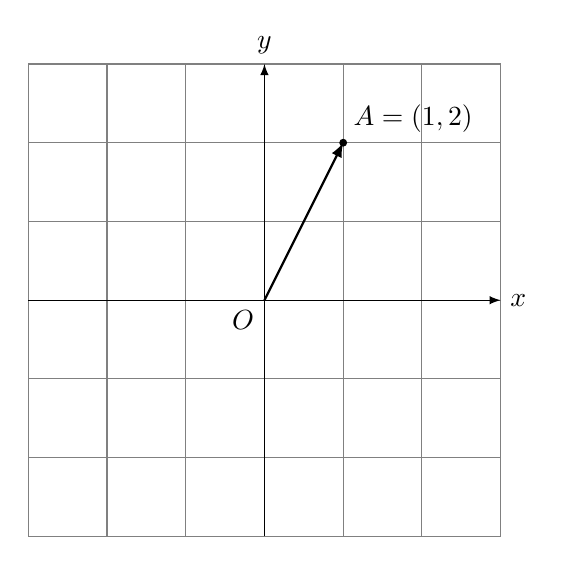
\begin{tikzpicture}
			\draw[gray] (-3,-3) grid (3,3);
			\draw[-latex] (-3,0) -- (3,0) node[right] {\(x\)};
			\draw[-latex] (0,-3) -- (0,3) node[above] {\(y\)};
			\draw[-latex, thick] (0,0) node[below left] {\(O\)} -- (1,2) node[above right] {\(A = (1,2)\)};
			\fill (1,2) circle (0.05);
		\end{tikzpicture}
		\caption{The position vector \(\protect\overrightarrow{OA}\) in \(\R^2\).}
		\label{fig:OA}
	\end{figure}
	We can write \(\overrightarrow{OA} = \cvec{1 \\ 2}\).
\end{eg}

\begin{defn}[Magnitude]
	The \textbf{magnitude} of a vector \(\vec{v} = a\vec{i} + b\vec{j} + c\vec{k}\) is defined as
	\[ \abs{\vec{v}} = \sqrt{a^2 + b^2 + c^2}. \] 
\end{defn}

\begin{eg}
	\label{eg:magnitude}
	The vector \(\vec{v} = \cvec{2 \\ 1 \\ 7}\) has a magnitude of 
	\[ \abs{\vec{v}} = \sqrt{2^2 + 1^2 + 7^2} = \sqrt{54} = 3 \sqrt{6}. \] 
\end{eg}

\subsection{Vector Operations}

\begin{defn}[Vector Addition]
	Let \(\vec{u} = \cvec{a \\ b \\ c}\) and \(\vec{v} = \cvec{d \\ e \\ f}\). 
	We define the \textbf{addition} of two vectors 
	\[\vec{u} + \vec{v} = \cvec{a + d \\ b + e \\ c + f}.\]
\end{defn}

\begin{defn}[Negative Vector] \label{defn:negv}
	Let \(\vec{v} = \cvec{a \\ b \\ c}\). 
	We define the \textbf{negative} of \(\vec{v}\), written as
	\[-\vec{v} = -\cvec{a \\ b \\ c} = \cvec{-a \\ -b \\ -c}.\]
\end{defn}

\begin{rmk}
	The subtraction of two vectors \(\vec{u} - \vec{v}\) is equivalent to writing \(\vec{u} + (-\vec{v})\). 
\end{rmk}

\begin{eg}
	Let \(\vec{u} = \cvec{1 \\ 2 \\ 3}\) and \(\vec{v} = \cvec{2 \\ 0 \\ -5}\). 
	Then
	\[ 
		\vec{u} + \vec{v} = \cvec{1 + 2 \\ 2 + 0 \\ 3 + (-5)} = \cvec{3 \\ 2 \\ -2},
		\qquad
		\vec{u} - \vec{v} = \cvec{1 - 2 \\ 2 - 0 \\ 3 - (-5)} = \cvec{-1 \\ 2 \\ 8}.
	\]
	\begin{figure}[H]
		\centering
		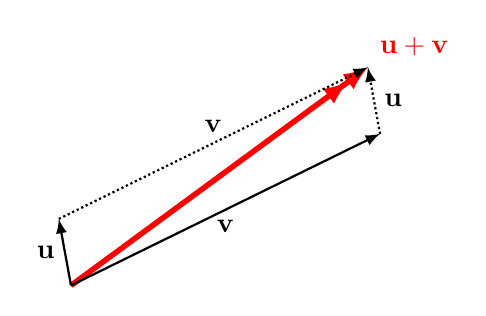
\begin{tikzpicture}
			\draw[-{latex}{latex}, line width=2pt, red] (0,0,0) -- (3,2,-2) node[above right] {\(\vec{u} + \vec{v}\)};
			\draw[-latex, thick] (0,0,0) -- (1,2,3) node[pos=0.5, left] {\(\vec{u}\)};
			\draw[-latex, thick] (0,0,0) -- (2,0,-5) node[pos=0.5, below] {\(\vec{v}\)};
			\draw[-latex, thick, densely dotted] (1,2,3) -- ++(2,0,-5) node[pos=0.5, above] {\(\vec{v}\)};
			\draw[-latex, thick, densely dotted] (2,0,-5) -- ++(1,2,3) node[pos=0.5, right] {\(\vec{u}\)};
		\end{tikzpicture}
		\caption{Vector addition.}
	\end{figure}
	\begin{figure}[H]
		\centering
		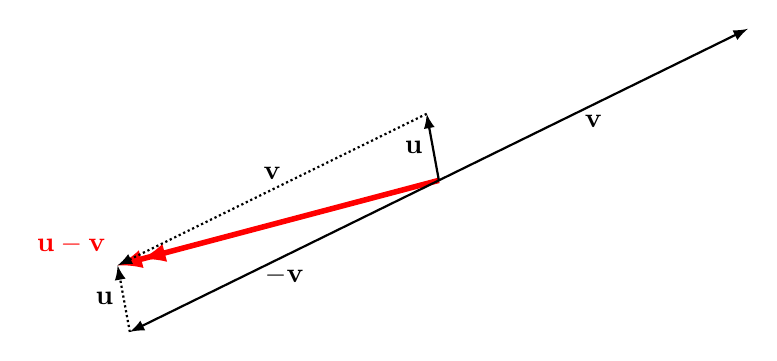
\begin{tikzpicture}
			\draw[-{latex}{latex}, line width=2pt, red] (0,0,0) -- (-1,2,8) node[above left] {\(\vec{u} - \vec{v}\)};
			\draw[-latex, thick] (0,0,0) -- (1,2,3) node[pos=0.5, left] {\(\vec{u}\)};
			\draw[-latex, thick] (0,0,0) -- (2,0,-5) node[pos=0.5, below] {\(\vec{v}\)};
			\draw[-latex, thick] (0,0,0) -- (-2,0,5) node[pos=0.5, below] {\(-\vec{v}\)};
			\draw[-latex, thick, densely dotted] (1,2,3) -- ++(-2,0,5) node[pos=0.5, above] {\(\vec{v}\)};
			\draw[-latex, thick, densely dotted] (-2,0,5) -- ++(1,2,3) node[pos=0.5, left] {\(\vec{u}\)};
		\end{tikzpicture}
		\caption{Vector subtraction.}
	\end{figure}
\end{eg}

We see from the above example a geometrical understanding of vector addition and subtraction.
To add two vectors, place the tail of the first vector to the tip of the second vector, then draw a vector from the tail of the first vector to the tip of the second vector.
Notice that which vector is added first does not matter---if you walked left three steps then walked forward five steps, it is the same as first walking forward five steps then walking left three steps.
\begin{defn}[Scalar Multiplication]
	Let \(\vec{v} = \cvec{a \\ b \\ c}\) and \(\lambda\) be a real number.
	We define the \textbf{scalar multiplication} of a vector
	\[\lambda \vec{v} = \lambda  \cvec{a \\ b \\ c} = \cvec{\lambda a \\ \lambda b \\ \lambda c}.\]
\end{defn}

Sometimes we may prefer to write a vector with a scalar ``factorised out''.
For example, 
\[ \frac{1}{3} \cvec{1 \\ 3 \\ 2} \text{ or } \frac{\cvec{1 \\ 3 \\ 2}}{3} \text{ looks better than } \cvec{\frac{1}{3} \\ 1 \\ \frac{2}{3}}. \] 

\begin{eg}
	\begin{enumerate}
		\item Let \(\vec{v} = \cvec{1 \\ 2 \\ 3}\).
		Then \(3\vec{v} = \cvec{3(1) \\ 3(2) \\ 3(3)} = \cvec{3 \\ 6 \\ 9}\).
		\item In \ref{defn:negv}, notice that \(\lambda = -1\).
	\end{enumerate}
	\begin{figure}[H]
		\centering
		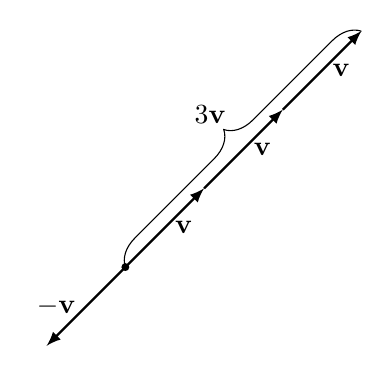
\begin{tikzpicture}
			\fill (0,0) circle (0.05);
			\draw[-latex, thick] (0,0) -- (1,1) node[pos=0.5, right] {\(\vec{v}\)};	
			\draw[-latex, thick] (1,1) -- (2,2) node[pos=0.5, right] {\(\vec{v}\)};	
			\draw[-latex, thick] (2,2) -- (3,3) node[pos=0.5, right] {\(\vec{v}\)};	
			\draw[decorate, decoration={brace, amplitude=10pt}] (0,0) -- (3,3) node[pos=0.5, above left, yshift=2mm, xshift=-1mm] {\(3\vec{v}\)};	
			\draw[-latex, thick] (0,0) -- (-1,-1) node[pos=0.5, left] {\(-\vec{v}\)};
		\end{tikzpicture}
	\end{figure}
\end{eg}

We see from the above example a geometrical understanding of scalar multiplication of a vector.
The scalar ``stretches'' the vector by a certain length.
We also see that a negative scalar flips the vector around.

\begin{exc}
	Draw, on the same diagram, a nonzero vector \(\vec{v}\) and \(\dfrac{1}{3}\vec{v}\).
\end{exc}

We can define the notion of parallel vectors based on this geometric intuition.

\begin{defn}[Parallel Vectors]
	Let \(\vec{u}\) and \(\vec{v}\) be vectors.
	We say that \(\vec{u}\) is \textbf{parallel} to \(\vec{v}\) if there exists a nonzero scalar \(\lambda\) such that 
	\[ \vec{u} = \lambda \vec{v}. \] 
\end{defn}


\begin{defn}[Displacement Vector]
	Let the points \(A\) and \(B\) be in \(\R^3\).
	Let \(O\) be the origin.
	The \textbf{displacement vector} between points \(A\) and \(B\) is \(\overrightarrow{AB}\), which is equal to
	\[ \overrightarrow{AB} = \overrightarrow{OB} - \overrightarrow{OA}. \] 
\end{defn}

We also define the notion of collinear points using displacement vectors and parallel vectors.

\begin{defn}
	Let \(A\), \(B\), and \(C\) be points.
	We say that \(A\), \(B\), and \(C\) are collinear if there exists a scalar \(\lambda\) such that 
	\[ \overrightarrow{AB} = \lambda \overrightarrow{BC}.\] 

	\begin{figure}[H]
		\centering
		\begin{tikzpicture}
			\node[above] at (2,1) (A) {\(A\)};
			\draw (2,1) -- (4,2) node[above] (B) {\(B\)};
			\draw (2,1) -- (6,3) node[above] (C) {\(C\)};
			\fill (2,1) circle (0.05);
			\fill (4,2) circle (0.05);
			\fill (6,3) circle (0.05);
		\end{tikzpicture}
	\end{figure}
\end{defn}

You can think that three points are collinear if a straight line can be drawn through them.

\begin{eg}
	Let the points \(A\) and \(B\) have coordinates \((1,2)\) and \((-1,1)\) respectively.
	\begin{figure}[H]
		\centering
		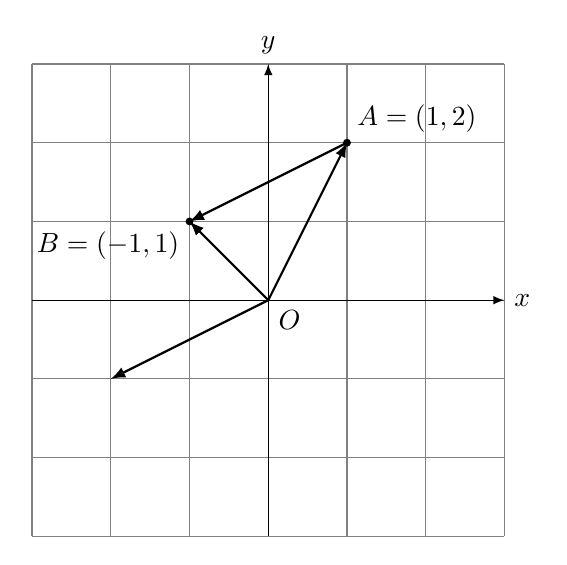
\begin{tikzpicture}
			\draw[gray] (-3,-3) grid (3,3);
			\draw[-latex] (-3,0) -- (3,0) node[right] {\(x\)};
			\draw[-latex] (0,-3) -- (0,3) node[above] {\(y\)};
			\draw[-latex, thick] (0,0) node[below right] {\(O\)} -- (1,2) node[above right] {\(A = (1,2)\)};
			\draw[-latex, thick] (0,0) -- (-1,1) node[below left] {\(B = (-1,1)\)};
			\draw[-latex, thick] (0,0) -- (-2,-1); 
			\fill (1,2) circle (0.05);
			\fill (-1,1) circle (0.05);
			\draw[-latex, thick] (1,2) -- (-1,1);
		\end{tikzpicture}
		\caption{Points \(A\), \(B\), and a few vectors.}
		\label{fig:OAB}
	\end{figure}
	Then the displacement vector \(\overrightarrow{AB} = \cvec{-1 \\ 1} - \cvec{1 \\ 2} = \cvec{-2 \\ -1}\). 
	The distance between the points \(A\) and \(B\) is simply \(\abs*{\overrightarrow{AB}}\), which is \(\sqrt{5}\).
\end{eg}

\begin{defn}[Zero Vector] \label{defn:zv}
	The \textbf{zero vector} is a vector of magnitude \(0\).
	It is written as \(\vec{0} = \cvec{0 \\ 0 \\ 0}\).
\end{defn}

\begin{prop}
	The zero vector is parallel to itself.
\end{prop}

\begin{proof}
	There must exist a nonzero scalar \(\lambda\) such that 
	\[ \cvec{0 \\ 0 \\ 0} = \lambda \cvec{0 \\ 0 \\ 0} \] 
	which is equivalent to solving the equation \(0 = 0 \lambda\).
	Any nonzero \(\lambda\) is a solution to this equation.
\end{proof}

\begin{defn}[Unit Vector]
	A \textbf{unit vector} is a vector of magnitude \(1\).
\end{defn}

\begin{thm}
	The unit vector of a vector \(\vec{v}\) is 
	\[ \vec{\hat{v}} = \frac{\vec{v}}{\abs{\vec{v}}}. \] 
\end{thm}

\begin{proof}
	We find out what is \(\displaystyle \abs*{\frac{\vec{v}}{\abs{\vec{v}}}}\).
	\begin{align*}
		\abs*{ \frac{\vec{v}}{\abs{\vec{v}}} } &= \abs*{ \left( \frac{1}{\abs{\vec{v}}} \vec{v} \right) } \\
											   &= \frac{1}{\abs{\vec{v}}} \abs{\vec{v}} \\
											   &= \frac{\abs{\vec{v}}}{\abs{\vec{v}}} \\
											   &= 1
	\end{align*}
	which fulfils the definition of a unit vector.
\end{proof}

\begin{eg}
	The unit vector of \(\vec{v}\) in Example \ref{eg:magnitude} is 
	\[ \vec{\hat{v}} = \frac{1}{\sqrt{54}} \cvec{2 \\ 1 \\ 7}. \] 
\end{eg}

\section{Dot and Cross Products}
\begin{defn}[Dot Product]
	Let \(\vec{u} = \cvec{a \\ b \\ c}\) and \(\vec{v} = \cvec{d \\ e \\ f}\).
	The \textbf{dot product} (or scalar product) \(\vec{u} \cdot \vec{v}\) is defined by
	\[ \vec{u} \cdot \vec{v} = ad + be + cf. \] 
	The following properties hold for any vectors \(\vec{u},\ \vec{v},\ \vec{w}\) and scalar \(\lambda\):
	\begin{enumerate}
		\item The dot product is commutative: \(\vec{u} \cdot \vec{v} = \vec{v} \cdot \vec{u}\).
		\item The dot product is distributive: \(\vec{u} \cdot (\vec{v} + \vec{w}) = \vec{u} \cdot \vec{v} + \vec{u} \cdot \vec{w}\).
		\item The dot product is associative with scalar multiplication: \(\vec{u} \cdot (\lambda \vec{v}) = \lambda (\vec{u} \cdot \vec{v}) = (\lambda \vec{u}) \cdot \vec{v}\). 
	\end{enumerate}
\end{defn}

\begin{thm}
	Let \(\vec{v}\) be a vector.
	Then 
	\[ \vec{v} \cdot \vec{v} = \abs{\vec{v}}^2. \] 
\end{thm}

\begin{proof}
	Let \(\vec{v} = \cvec{a \\ b \\ c}\). Then
	\[ \vec{v} \cdot \vec{v} = \cvec{a \\ b \\ c} \cdot \cvec{a \\ b \\ c} = a^2 + b^2 + c^2 = \abs{\vec{v}}^2. \] 
\end{proof}

\begin{defn}[Angle Between Two Vectors]
	Let \(\vec{u}\) and \(\vec{v}\) be vectors with their tails placed together (refer to figure).
	We define the \textbf{angle between two vectors} \(\vec{u}\) and \(\vec{v}\) to be \(\theta\), where \(\theta\) is the smaller angle of the two.
	\begin{figure}[H]
		\centering
		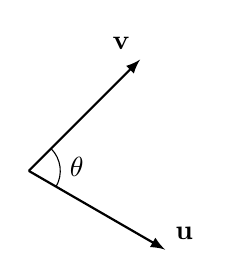
\begin{tikzpicture}
			\draw[-latex, thick] (0,0) -- (-30:2) node[above right]{\(\vec{u}\)};
			\draw[-latex, thick] (0,0) -- (45:2) node[above left]{\(\vec{v}\)};
			\draw (-30:0.4) arc (-30:45:0.4) node[pos=0.5, right] {\(\theta\)};
		\end{tikzpicture}
	\end{figure}
	The definition also holds if their tips \((\rightarrow)\) are placed togehter.
\end{defn}

\begin{disc}
	Consider two points \(A\) and \(B\) with respect to an origin \(O\). 
	Let them have position vectors \(\vec{a}\) and \(\vec{b}\) respectively, separated by an angle \(\theta\).
	\begin{figure}[H]
		\centering
		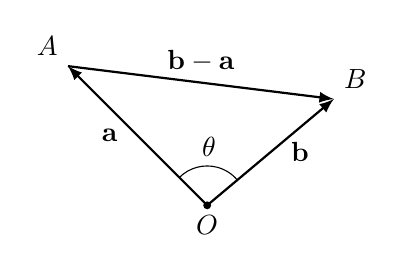
\begin{tikzpicture}
			\fill (0,0) circle (0.05) node[below] (O) { \(O\) };
			\draw[-latex, thick] (0,0) -- (135:2.5) node[above left] (A) { \(A\) };
			\draw[-latex, thick] (0,0) -- (40:2.1) node[above right] (B) { \(B\) };
			\draw[-latex, thick] (135:2.5) -- (40:2.1) node[pos=0.5, above] {\(\vec{b} - \vec{a}\)};
			\node[left] at ($(O)!0.5!(A)$) { \(\vec{a}\) };
			\node[right] at ($(O)!0.5!(B)$) { \(\vec{b}\) };
			\draw (135:0.5) arc (135:40:0.5) node[above, pos=0.5] {\(\theta\)};
		\end{tikzpicture}
	\end{figure}
	By the law of cosines,
	\begin{align*}
		 \abs{\vec{b} - \vec{a}}^2 &= \abs{\vec{a}}^2 + \abs{\vec{b}}^2 - 2 \abs{\vec{a}} \abs{\vec{b}} \cos \theta  \\
		  (\vec{b} - \vec{a}) \cdot (\vec{b} - \vec{a}) &= (\vec{a} \cdot \vec{a}) + (\vec{b} \cdot \vec{b}) - 2 \abs{\vec{a}} \abs{\vec{b}} \cos \theta \\
		  \cancel{(\vec{a} \cdot \vec{a})} - 2 (\vec{a} \cdot \vec{b}) + \cancel{(\vec{b} \cdot \vec{b})} &= \cancel{(\vec{a} \cdot \vec{a})} + \cancel{(\vec{b} \cdot \vec{b})} - 2 \abs{\vec{a}} \abs{\vec{b}} \cos \theta \\
		  \cancel{-2} (\vec{a} \cdot \vec{b}) &= \cancel{-2} \abs{\vec{a}} \abs{\vec{b}} \cos \theta \\
		  \vec{a} \cdot \vec{b} &= \abs{\vec{a}} \abs{\vec{b}} \cos \theta.
	\end{align*}
\end{disc}

\begin{defn}[Geometric Dot Product] \label{defn:gdpdt}
	Let \(\vec{u}\) and \(\vec{v}\) be vectors separated by an angle \(0^\circ \leq \theta \leq 180^\circ\).
	The \textbf{dot product} is also defined as 
	\[ \vec{u} \cdot \vec{v} = \abs{\vec{u}} \abs{\vec{v}} \cos \theta. \] 
\end{defn}

\begin{thm} \label{thm:perptest}
	Let \(\vec{u}\) and \(\vec{v}\) be vectors separated by an angle \(\theta\).
	Then
	\[ \vec{u} \cdot \vec{v} = 0 \iff 
		\begin{cases}
			\vec{u} = \vec{0}, \text{ or} \\
			\vec{v} = \vec{0}, \text{ or} \\
			\theta = 90^\circ.
		\end{cases}
	\] 
\end{thm}

\begin{proof}
	\((\Rightarrow)\) By Definition \ref{defn:gdpdt}, we have
	\[ \vec{u} \cdot \vec{v} = \abs{\vec{u}} \abs{\vec{v}} \cos \theta = 0\] 
	which implies either \(\abs{\vec{u}}\), \(\abs{\vec{v}}\), or \(\cos \theta\) is equal to zero.
	By Definition \ref{defn:zv}, \(\abs{\vec{u}} = 0 \implies \vec{u} = \vec{0}\). 
	A similar argument can be made for \(\vec{v}\).
	For \(\cos \theta = 0\), the only solution in \(0^\circ \leq \theta \leq 180^\circ\) is \(\theta = 90^\circ\), which means that \(\vec{u}\) and \(\vec{v}\) are perpendicular.

	\((\Leftarrow)\) If \(\vec{u} = \vec{0}\) and \(\vec{v} = \cvec{d \\ e \\ f}\), then the dot product will be 
	\[ \vec{0} \cdot \vec{v} = 0(d) + 0(e) + 0(f) = 0. \] 
	A similar argument can be made if \(\vec{v} = \vec{0}\).
	If \(\vec{u}\) and \(\vec{v}\) are perpendicular to each other, then the angle between them is \(90^\circ\).
	By Definition \ref{defn:gdpdt}, we have 
	\[ \vec{u} \cdot \vec{v} = \abs{\vec{u}} \abs{\vec{v}} \cos 90^\circ = \abs{\vec{u}} \abs{\vec{v}} (0) = 0. \] 
	This concludes the proof.
\end{proof}


\begin{defn}[Cross Product]
	Let \(\vec{u} = \cvec{a \\ b \\ c}\) and \(\vec{v} = \cvec{d \\ e \\ f}\).
	The \textbf{cross product} (or vector product) \(\vec{u} \times \vec{v}\) is defined by
	\[ \vec{u} \times \vec{v} = \cvec{bf - ce \\ cd - af \\ ae - bd}.  \] 
	The following properties hold, for any vectors \(\vec{u}\), \(\vec{v}\), \(\vec{w}\) and scalar \(\lambda\),
	\begin{enumerate}
		\item The cross product is anti-commutative: \(\vec{u} \times \vec{v} = -\vec{v} \times \vec{u}\).
		\item The cross product is distributive: \(\vec{u} \times (\vec{v} + \vec{w}) = \vec{u} \times \vec{v} + \vec{u} \times \vec{w}\). 
		\item The cross product is associative with scalar multiplication: \((\lambda \vec{u}) \times \vec{v} = \lambda (\vec{u} \times \vec{v}) = \vec{u} \times (\lambda \vec{v})\).
	\end{enumerate}
\end{defn}

\begin{thm}
	Let \(\vec{v}\) be a vector.
	Then 
	\[ \vec{v} \times \vec{v} = \vec{0}. \] 
\end{thm}

\begin{proof}
	Let \(\vec{v} = \cvec{a \\ b \\ c}\).
	Then 
	\[ \vec{v} \times \vec{v} = \cvec{a \\ b \\ c} \times \cvec{a \\ b \\ c} = \cvec{bc - cb \\ ac - ca \\ ab - ba} = \cvec{0 \\ 0 \\ 0} = \vec{0}. \] 
\end{proof}

\begin{defn}[Geometric Cross Product] \label{defn:gcpdt}
	Let \(\vec{u}\) and \(\vec{v}\) be vectors separated by an angle \(0^\circ \leq \theta \leq 180^\circ\).
	The \textbf{cross product} is also defined as 
	\[ \vec{u} \times \vec{v} = \left( \abs{\vec{u}} \abs{\vec{v}} \sin \theta \right) \vec{\hat{n}} \] 
	where \(\vec{\hat{n}}\) is the unit vector that is perpendicular to the two vectors \(\vec{u}\) and \(\vec{v}\), and its direction is determined by the right hand rule.
\end{defn}

\begin{prop}
	Let \(\vec{u}\) and \(\vec{v}\) be vectors separated by an angle \(\theta\).
	The magnitude of the vector \(\vec{u} \times \vec{v}\) is 
	\[\abs{\vec{u} \times \vec{v}} = \abs{\vec{u}} \abs{\vec{v}} \sin \theta.\]
\end{prop}

\begin{proof}
	It is obvious.
	By Definition \ref{defn:gcpdt}, since \(\vec{\hat{n}}\) has a magnitude of \(1\), whatever the scalar is is going to be the magnitude. 
\end{proof}

\begin{thm}
	Let \(\vec{u}\) and \(\vec{v}\) be vectors separated by an angle \(\theta\).
	Then
	\[ \vec{u} \times \vec{v} = \vec{0} \iff 
		\begin{cases}
			\vec{u} = \vec{0}, \text{ or} \\
			\vec{v} = \vec{0}, \text{ or} \\
			\theta = 0^\circ \text{ or } 180^\circ.
		\end{cases}
	\] 
\end{thm}

\begin{proof}
	\((\Rightarrow)\) By Definition \ref{defn:gcpdt}, we have
	\[ \vec{u} \times \vec{v} = (\abs{\vec{u}} \abs{\vec{v}} \sin \theta) \vec{\hat{n}} = \vec{0} \] 
	which means \(\abs{\vec{u}}\), \(\abs{\vec{v}}\), or \(\sin \theta\) is equal to zero.
	By Definition \ref{defn:zv}, \(\abs{\vec{u}} = 0 \implies \vec{u} = \vec{0}\). 
	A similar argument can be made for \(\vec{v}\).
	For \(\sin \theta = 0\), this is true when \(\theta = 0^\circ\) or \(\theta = 180^\circ\).
	Any of these conditions would also mean that the direction of vector \(\vec{\hat{n}}\) is not well-defined.

	\((\Leftarrow)\) If \(\vec{u} = \vec{0}\) and \(\vec{v} = \cvec{d \\ e \\ f}\), then the cross product will be 
	\[ \vec{u} \times \vec{v} = \cvec{0f - 0e \\ 0d - 0f \\ 0e - 0d} = \cvec{0 \\ 0 \\ 0} = \vec{0}.  \] 
	A similar argument can be made if \(\vec{v} = \vec{0}\).
	If \(\vec{u}\) and \(\vec{v}\) are parallel to each other, then the angle between them is \(0^\circ\) or \(180^\circ\).
	Without loss of generality, since \(\sin 0^\circ = \sin 180^\circ\), we consider \(\theta = 0^\circ\). 
	By Definition \ref{defn:gcpdt}, we have 
	\[ \vec{u} \cdot \vec{v} = ( \abs{\vec{u}} \abs{\vec{v}} \sin 0^\circ ) \vec{\hat{n}} = ( \abs{\vec{u}} \abs{\vec{v}} (0) ) \vec{\hat{n}} = \vec{0}. \] 
	This concludes the proof.
\end{proof}


\section{Vector Geometry}
In this section we will learn how to use vectors to solve problems in geometry.

\subsection{Areas of Shapes}
\begin{disc}
	Consider triangle \(ABC\).
	\begin{figure}[H]
		\centering
		\begin{tikzpicture}
			\draw (0,0) node[below] (a) {\(A\)} -- (-1,3) node[left] (b) {\(B\)} -- (2,2) node[right] (c) {\(C\)} -- cycle;
			\node[left] at ($(a)!0.5!(b)$) {\(c\)};
			\node[above] at ($(b)!0.5!(c)$) {\(a\)};
			\node[right] at ($(a)!0.5!(c)$) {\(b\)};
		\end{tikzpicture}
	\end{figure}
	Recall that its area will be 
	\[ \text{area} = \frac{1}{2} a b \sin \angle BCA. \] 
	Notice this takes a very similar form to the cross product in Definition \ref{defn:gcpdt}.
	If we considered the edges of this traingle to be made up of vectors, then we can also write
	\[ \text{area} = \frac{1}{2} \abs*{\overrightarrow{AC}} \abs*{\overrightarrow{BC}} \sin \angle BCA \] 
	which is also equivalent to
	\[ \text{area} = \frac{1}{2} \abs*{\overrightarrow{AC} \times \overrightarrow{BC}}. \] 
\end{disc}

\begin{thm}
	Let \(A\), \(B\), and \(C\) be three non-collinear points such that they form triangle \(ABC\).
	The area of triangle \(ABC\) is then equal to
	\[ \text{area} = \frac{1}{2} \abs*{\overrightarrow{AC} \times \overrightarrow{BC}}. \] 
\end{thm}

\begin{thm}
	Let \(A\), \(B\), \(C\), and \(D\) be four non-collinear points, where \(AB \parallel DC\) and \(AD \parallel BC\) such that they form parallelogram \(ABCD\).
	The area of parallelogram \(ABCD\) is then equal to
	\[ \text{area} = \abs*{\overrightarrow{AB} \times \overrightarrow{AD}}. \] 
	\begin{figure}[H]
		\centering
		\begin{tikzpicture}
			\draw (0,0) node[below left] {\(A\)} -- (3,0) node[below right] {\(B\)} -- (4,2) node[above right] {\(C\)} -- (1,2) node[above left] {\(D\)} -- cycle;
		\end{tikzpicture}
	\end{figure}
\end{thm}

\begin{proof}
	Exercise (\textit{Hint: Show that triangle \(ABD\) and triangle \(CBD\) are congruent}).
\end{proof}

\subsection{Ratio Theorem}
\begin{thm}[Ratio Theorem]
	With respect to the origin \(O\), let \(A\) and \(B\) be distinct points with position vectors \(\vec{a}\) and \(\vec{b}\) respectively.
	Let point \(P\) lie on the line \(AB\) such that \(AP : PB = \lambda : \mu\), where \(\lambda\) and \(\mu\) are positive real numbers.
	Then the position vector of \(P\), \(\vec{p}\), is 
	\[ \vec{p} = \frac{\mu \vec{a} + \lambda \vec{b}}{\lambda + \mu}. \] 
\end{thm}

\begin{figure}[H]
	\centering
	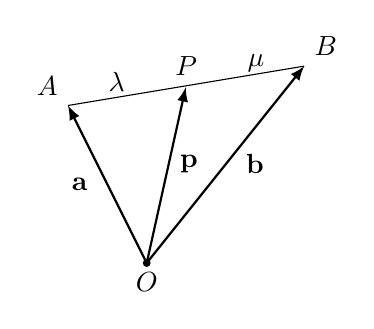
\begin{tikzpicture}
		\fill (0,0) circle (0.05) node[below] (O) {\(O\)};
		\draw[-latex, thick] (0,0) -- (-1,2) node[above left] (A) {\(A\)};
		\draw[-latex, thick] (0,0) -- (2,2.5) node[above right] (B) {\(B\)};
		\node[left] at ($(O)!0.5!(A)$) {\(\vec{a}\)};
		\node[right] at ($(O)!0.5!(B)$) {\(\vec{b}\)};
		\draw (-1,2) -- (2,2.5) node[pos=0.5, inner sep=0, outer sep=0] (P) {};
		\draw[-latex, thick] (0,0) -- (P) node[above] {\(P\)};
		\node[right] at ($(O)!0.6!(P)$) {\(\vec{p}\)};
		\node[above, yshift=-2mm] at ($(A)!0.5!(P)$) {\(\lambda\)};
		\node[above, yshift=-2mm] at ($(P)!0.5!(B)$) {\(\mu\)};
	\end{tikzpicture}
\end{figure}

\begin{proof}
	Since \(AP : PB = \lambda : \mu\), we can write
	\[ \frac{AP}{PB} = \frac{\abs*{\overrightarrow{AP}}}{\abs*{\overrightarrow{PB}}} = \frac{\abs{\vec{p} - \vec{a}}}{\abs{\vec{b} - \vec{p}}} = \frac{\lambda}{\mu}. \] 
	Rearranging, we get 
	\[ \mu|\vec{p} - \vec{a}| = \lambda |\vec{b} - \vec{p}|. \] 
	But since \(\vec{p} - \vec{a}\) and \(\vec{b} - \vec{p}\) are in the same direction, 
	\[ \mu(\vec{p} - \vec{a}) = \lambda (\vec{b} - \vec{p}). \]
	With a bit of manipulation,
	\begin{align*}
		\mu \vec{p} - \mu \vec{a} &= \lambda \vec{v} - \lambda \vec{p} \\
		\mu \vec{p} + \lambda \vec{p} &= \lambda \vec{b} + \mu \vec{a} \\
		(\mu + \lambda) \vec{p} &= \mu \vec{a} + \lambda \vec{b} \\
		\vec{p} &= \frac{\mu \vec{a} + \lambda \vec{b}}{\mu + \lambda}.
	\end{align*}
	This concludes the proof.
\end{proof}

\section{Lines}
\begin{disc}\label{disc:line}
	Recall that the general formula for a straight line in \(\R^2\) can be expressed in the form
	\[ y = mx + c \] 
	where \(m\) and \(c\) represent the gradient and \(y\)-intercept respectively.

	What about a line in \(\R^3\)?

	Let us consider a position vector \(\vec{a}\) of a point \(A\) in the line \(\ell\) and a vector \(\vec{m}\) that is \emph{parallel} to \(\ell\).

	\begin{figure}[H]
		\centering
		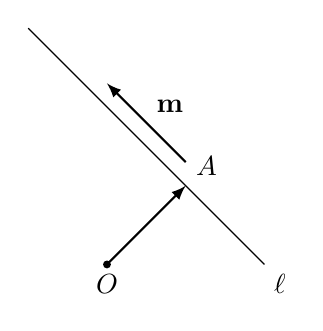
\begin{tikzpicture}
			\draw[-latex, thick] (0,0) node[below] {\(O\)} -- (1,1) node[above right] {\(A\)};
			\draw (-1,3) -- (2,0) node[below right] {\(\ell\)};
			\draw[latex-, thick] (0,2.3) -- (1,1.3) node[above right, pos=0.5] {\(\vec{m}\)};
			\fill (0,0) circle (0.05);
		\end{tikzpicture}
		\caption{A line \(\ell\) that passes through \(A\) and is parallel to \(\vec{m}\).}
	\end{figure}

	Notice that \(\vec{a} + \vec{m}\) would give us the position vector of some point on the line. 
	If we let \(\vec{m}\) be multiplied by some scalar \(\lambda\), then \(\vec{a} + \lambda \vec{m}\) will be some position vector also on the line.

	\begin{figure}[H]
		\centering
		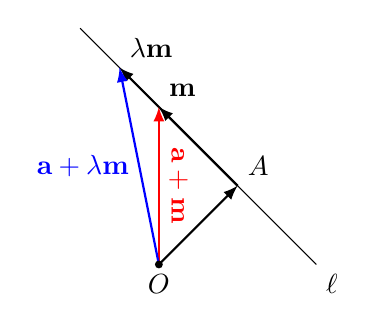
\begin{tikzpicture}
			\draw[-latex, thick] (0,0) node[below] {\(O\)} -- (1,1) node[above right] {\(A\)};
			\draw (-1,3) -- (2,0) node[below right] {\(\ell\)};
			\draw[latex-, thick] (0,2) -- (1,1) node[above right, pos=0] {\(\vec{m}\)};
			\draw[latex-, thick] (-0.5,2.5) -- (1,1) node[above right, pos=0] {\(\lambda \vec{m}\)};
			\draw[-latex, thick, red] (0,0) -- (0,2) node[rotate=270, pos=0.5, above] {\(\vec{a} + \vec{m}\)};
			\draw[-latex, thick, blue] (0,0) -- (-0.5,2.5) node[pos=0.5, left] {\(\vec{a} + \lambda \vec{m}\)};
			\fill (0,0) circle (0.05);
		\end{tikzpicture}
		\caption{How we can use vector addition to ``reach'' the points in a line.}
	\end{figure}

	In fact, if we let the equation ``run'' through all possible values for \(\lambda \in \R\), we can eventually reach every point on the line \(\ell\).
	\begin{figure}[H]
		\centering
		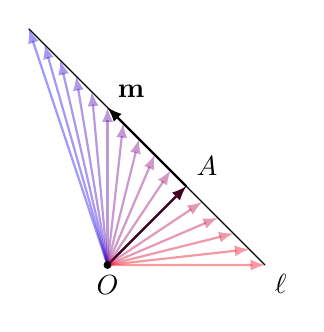
\begin{tikzpicture}
			\draw[-latex, thick] (0,0) node[below] {\(O\)} -- (1,1) node[above right] {\(A\)};
			\draw (-1,3) -- (2,0) node[below right] {\(\ell\)};
			\draw[latex-, thick] (0,2) -- (1,1) node[above right, pos=0] {\(\vec{m}\)};
			\foreach[count=\i] \x in {-1, -0.8, -0.6, -0.4, -0.2, 0, 0.2, 0.4, 0.6, 0.8, 1, 1.2, ..., 2}{
				\pgfmathsetmacro\k{\i * 6} 
				\draw[-latex, color=red!\k!blue, opacity=0.4, thick] (0,0) -- (\x, {-\x + 2});};
			\fill (0,0) circle (0.05);
		\end{tikzpicture}
		\caption{A few of the possible \(\vec{a} + \lambda \vec{m}\) for some real values of \(\lambda\).}
	\end{figure}
	All these points that can be reached with this vector equation form the line \(\ell\).
	This means we can describe the line \(\ell\) such that it is the \emph{union} of all these points with position vectors that can be expressed in the form \(\vec{a} + \lambda \vec{m}\), where \(\lambda \in \R\) (see Definition \ref{defn:line}).

	In some sense, \(m\) in the equation \(y = mx + c\) is very similar to \(\lambda \vec{m}\), because it tells you what is the ``gradient'' of the line.
	We call \(\vec{m}\) the \textbf{direction vector} of the line \(\ell\).
	Furthermore, \(\vec{a}\) also is analogous to \(c\) in \(y = mx + c\), as it tells you a ``fixed'' point the line definitely passes though.
\end{disc}

\begin{defn}[Vector Equation of a Line] \label{defn:line}
	A \textbf{line} \(\ell\) that 
	\begin{enumerate}
		\item passes though a point with position vector \(\vec{a}\), and
		\item is parallel to a vector \(\vec{m}\), called the \textbf{direction vector},
	\end{enumerate}
	has the \textbf{vector equation}
	\[ \ell \colon \vec{r} = \vec{a} + \lambda \vec{m}, \quad \lambda \in \R \] 
	where \(\vec{r}\) denotes the position vector of a point in \(\ell\). 
\end{defn}

\begin{eg}
	The set of points with position vector \(\vec{r}\) satisfy the equation
	\[ \ell \colon \vec{r} = \cvec{1 \\ 2 \\ 1} + \lambda \cvec{3 \\ 1 \\ 2}, \quad \lambda \in \R \] 
	form the line \(\ell\).
	\begin{enumerate}
		\item The point \((1, 2, 1)\) is on the line \(\ell\) when \(\lambda = 0\).
		\item The point \((4, 3, 3)\) is on the line \(\ell\) when \(\lambda = 1\).
		\item The point \((0, 1, 0)\) is \emph{not} on the line \(\ell\), as there is no value for \(\lambda\) such that \(\vec{r} = \cvec{0 \\ 1 \\ 0}\).
	\end{enumerate}
\end{eg}

From Definition \ref{defn:line}, we can write it out with column vectors as 
\[ \ell \colon \cvec{x \\ y \\ z} = \cvec{a_1 \\ a_2 \\ a_3} + \lambda \cvec{m_1 \\ m_2 \\ m_3} \implies \cvec{x \\ y \\ z} = \cvec{a_1 + \lambda m_1 \\ a_2 + \lambda m_2 \\ a_3 + \lambda m_3} \implies 
\begin{cases}
	x = a_1 + \lambda m_1, \\
	y = a_2 + \lambda m_2, \\
	z = a_3 + \lambda m_3.
\end{cases}\] 
The set of three equations for \(x, y, z\) also can define the line \(\ell\).

\begin{defn}[Parametric Equation of a Line] \label{defn:linep}
	From the above derivation, the line \(\ell\) can be expressed in its \textbf{parametric equation} as
	\[ \ell \colon 
	\begin{cases}
		x = a_1 + \lambda m_1, \\
		y = a_2 + \lambda m_2, \\
		z = a_3 + \lambda m_3.
	\end{cases}\] 
	where \(\lambda \in \R\).
\end{defn}
From Definition \ref{defn:linep}, we can set \(\lambda\) as the subject, yielding
\[ \lambda = \frac{x - m_1}{a_1} = \frac{y - m_2}{a_2} = \frac{z - m_3}{a_3} \] 
which also has enough information to tell us about the line \(\ell\).
\begin{defn}[Cartesian Equation of a Line]
	\begin{enumerate}
		\item The line \(\ell\) can also be expressed in the \textbf{Cartesian form}:
		\[ \ell \colon \frac{x - m_1}{a_1} = \frac{y - m_2}{a_2} = \frac{z - m_3}{a_3} \] 
		for nonzero \(m_1\), \(m_2\), or \(m_3\).
		\item If \(m_1\) or \(m_2\) or \(m_3\) is equal to zero, then \(x = m_1\) or \(y = m_2\) or \(z = m_3\).
	\end{enumerate}
\end{defn}

\begin{eg}
	The line \(\ell\) is defined by
	\[ \ell \colon \vec{r} = \cvec{0 \\ 1 \\ 3} + \lambda \cvec{2 \\ 0 \\ 1}, \quad \lambda \in \R. \]
	Express \(\ell\) in the parametric and Cartesian forms.
	\begin{soln}
		Based on Definition \ref{defn:linep}, 
		\[ \ell \colon 
		\begin{cases}
			x = 2 \lambda, \\
			y = 1, \\
			z = 3 + \lambda.
		\end{cases}\] 
		where \(\lambda \in \R\).

		For the Cartesian form, we have
		\[ \ell \colon \frac{x}{2} = \frac{z - 3}{1}, y = 1. \] 
	\end{soln}
\end{eg}

\section{Planes}
\begin{disc}
	Let us revisit Discussion \ref{disc:line}.

	We know that we can define a line \(\ell\) in an equation of the form 
	\[ \ell \colon \vec{r} = \vec{a} + \lambda \vec{m_1}, \quad \lambda \in \R. \] 

	\begin{figure}[H]
		\centering
		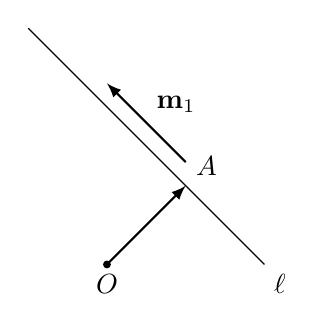
\begin{tikzpicture}
			\draw[-latex, thick] (0,0) node[below] {\(O\)} -- (1,1) node[above right] {\(A\)};
			\draw (-1,3) -- (2,0) node[below right] {\(\ell\)};
			\draw[latex-, thick] (0,2.3) -- (1,1.3) node[above right, pos=0.5] {\(\vec{m}_1\)};
			\fill (0,0) circle (0.05);
		\end{tikzpicture}
		\caption{A line \(\ell\) that passes through the point \(A\) with position vector \(\vec{a}\) and is parallel to \(\vec{m}_1\).}
	\end{figure}

	Let us add another vector \(\vec{m}_2\) that is not parallel to \(\vec{m}_1\). 
	What happens now?

	\begin{figure}[H]
		\centering
		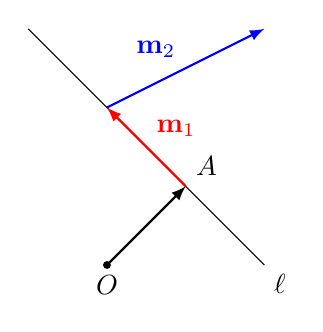
\begin{tikzpicture}
			\draw[-latex, thick] (0,0) node[below] {\(O\)} -- (1,1) node[above right] {\(A\)};
			\draw (-1,3) -- (2,0) node[below right] {\(\ell\)};
			\draw[latex-, red, thick] (0,2) -- (1,1) node[above right, pos=0.5] {\(\vec{m}_1\)};
			\draw[-latex, blue, thick] (0,2) -- (2,3) node[above left, pos=0.5] {\(\vec{m}_2\)};
			\fill (0,0) circle (0.05);
		\end{tikzpicture}
		\caption{The diagram for \(\vec{a} + \vec{m}_1 + \vec{m}_2\).}
	\end{figure}
	Let us consider the equation
	\[ \vec{a} + \lambda \vec{m}_1 + \mu \vec{m}_2\]
	where \(\lambda\) and \(\mu\) are real numbers.
	We fix \(\mu = 1\) for now, and look at what happens when \(\lambda\) varies.
	We can trace out a line that is parallel to the original line \(\ell\).

	\begin{figure}[H]
		\centering
		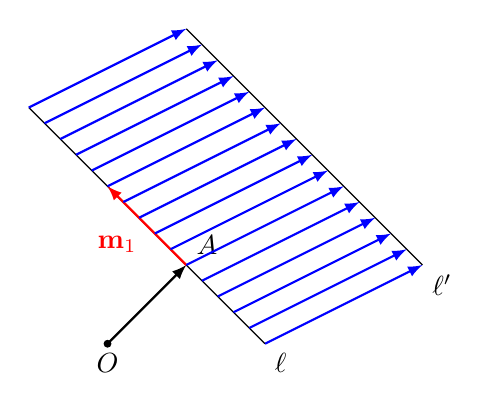
\begin{tikzpicture}
			\draw[-latex, thick] (0,0) node[below] {\(O\)} -- (1,1) node[above right] {\(A\)};
			\draw (-1,3) -- (2,0) node[below right] {\(\ell\)};
			\draw (1,4) -- (4,1) node[below right] {\(\ell'\)};
			\draw[latex-, red, thick] (0,2) -- (1,1) node[below left, pos=0.5] {\(\vec{m}_1\)};
			\foreach[count=\i] \x in {-1, -0.8, -0.6, -0.4, -0.2, 0, 0.2, 0.4, 0.6, 0.8, 1, 1.2, ..., 2}{
				\draw[-latex, blue, thick] (\x,{-\x + 2}) -- ++(2,1);
			}
			\fill (0,0) circle (0.05);
		\end{tikzpicture}
		\caption{For various \(\lambda\) and a fixed \(\mu\), we can trace out \(\ell'\).}
	\end{figure}

	Now let's set \(\mu = 2\).
	This is equivalent to stretching out all the blue arrows in the figure by a factor of two.
	\begin{figure}[H]
		\centering
		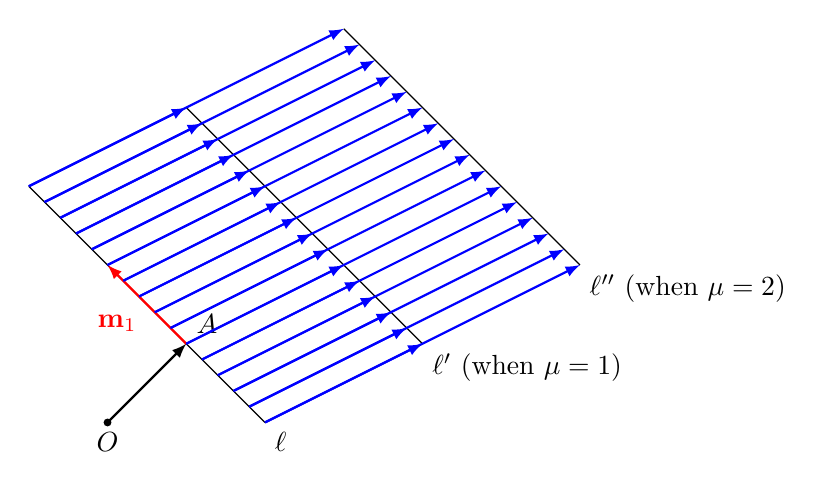
\begin{tikzpicture}
			\draw[-latex, thick] (0,0) node[below] {\(O\)} -- (1,1) node[above right] {\(A\)};
			\draw (-1,3) -- (2,0) node[below right] {\(\ell\)};
			\draw (1,4) -- (4,1) node[below right] {\(\ell'\) (when \(\mu = 1\))};
			\draw (3,5) -- (6,2) node[below right] {\(\ell''\) (when \(\mu = 2\))};
			\draw[latex-, red, thick] (0,2) -- (1,1) node[below left, pos=0.5] {\(\vec{m}_1\)};
			\foreach[count=\i] \x in {-1, -0.8, -0.6, -0.4, -0.2, 0, 0.2, 0.4, 0.6, 0.8, 1, 1.2, ..., 2}{
				\draw[-latex, blue, thick] (\x,{-\x + 2}) -- ++(2,1);
			}
			\foreach[count=\i] \x in {-1, -0.8, -0.6, -0.4, -0.2, 0, 0.2, 0.4, 0.6, 0.8, 1, 1.2, ..., 2}{
				\draw[-latex, blue, thick] (\x,{-\x + 2}) -- ++(4,2);
			}
			\fill (0,0) circle (0.05);
		\end{tikzpicture}
		\caption{Changing \(\mu\), we can get more lines but also parallel to \(\ell\).}
	\end{figure}
	
	We can repeat this for all values of \(\mu\).
	Eventually, we get a lot of lines that are parallel to \(\ell\).
	The \emph{union} of all these lines  will form a plane.
\end{disc}

\begin{defn}[Vector Equation of a Plane]
	A line \(p\) that 
	\begin{enumerate}
		\item contains a point with position vector \(\vec{a}\), and
		\item contains two non-parallel vectors \(\vec{m}_1\) and \(\vec{m_2}\),
	\end{enumerate}
	has the \textbf{vector equation}
	\[ p \colon \vec{r} = \vec{a} + \lambda \vec{m}_1 + \mu \vec{m}_2, \quad \lambda, \mu \in \R \] 
	where \(\vec{r}\) denotes the position vector of a point in \(p\).
\end{defn}

\begin{disc}
	Illustrated in Figure \ref{fig:dpplane}, the plane \(p\) contains a \emph{fixed} point \(A\) with position vector \(\vec{a}\), \emph{any} point \(R\) with position vector \(r\), and a vector \(\vec{n}\) that is perpendicular to \(p\).
	\begin{figure}[H] 
		\centering
		\begin{tikzpicture}[x={(0:1cm)}, y={(45:1cm)}, z={(90:1cm)}]
			\draw (-4, -2, 5) -- (-4, 2, 5) -- (4, 2, 5) node[right] {\(p\)} -- (4, -2, 5) -- cycle;
			\draw[thick, -latex] (0, 0, 0) node[below] {\(O\)}-- (1, 1, 5) node[pos=0.5, right] {\(\vec{r}\)};
			\draw[thick, -latex] (0, 0, 0) -- (-3, -1, 5) node[pos=0.5, left] {\(\vec{a}\)};
			\draw[dashed] (-3, -1, 5) node[left] {\(A\)} -- (1, 1, 5) node[right] {\(R\)};
			\draw[thick, -latex] (3.5, 1.9, 5) -- (3.5, 1.9, 6) node[right] {\(\vec{n}\)};
		\end{tikzpicture}
		\caption{Plane \(p\) that contains \(A\), \(R\), and is perpendicular to \(\vec{n}\).}
		\label{fig:dpplane}
	\end{figure}

	We look at the vector \(\overrightarrow{AR} = \vec{r} - \vec{a}\).
	Since \(\overrightarrow{AR}\) is perpendicular to \(\vec{n}\), by Theorem \ref{thm:perptest}, 
	\begin{align*}
		\overrightarrow{AR} \cdot \vec{n} = (\vec{r} - \vec{a}) \cdot \vec{n} &= 0 \\
		\iff \vec{r} \cdot \vec{n} - \vec{a} \cdot \vec{n} &= 0 \\
		\iff \vec{r} \cdot \vec{n} &= \vec{a} \cdot \vec{n}.
	\end{align*}
	But \(\vec{a}\) is fixed (or rather, known), so \(\vec{a} \cdot \vec{n}\) can be replaced by some number \(D\).
	\[ \vec{r} \cdot \vec{n} = D. \] 
	This means that any point \(R\) with position vector \(\vec{r}\) is contained in \(p\) if the dot product \(\vec{r} \cdot \vec{n} = D\).
	We call this the dot product form of the equation of a plane.
\end{disc}

\begin{defn}[Dot Product Equation of a Plane]
	Let \(p\) be a plane that contains a point with position vector \(\vec{a}\) and is perpendicular to the vector \(\vec{n}\).
	Then we can write its \textbf{dot product equation}
	\[ p \colon \vec{r} \cdot \vec{n} = \vec{a} \cdot \vec{n} \] 
	where \(\vec{r}\) is the position vector of any point in \(p\).
\end{defn}


\end{document}
